\documentclass[11pt]{article}
\usepackage[margin=1in]{geometry}
\usepackage{graphicx}
\usepackage{listings}
\usepackage{color}
\usepackage{amsmath}

% Define custom colors for MATLAB code
\definecolor{mygreen}{rgb}{0,0.6,0}
\definecolor{mygray}{rgb}{0.5,0.5,0.5}
\definecolor{mymauve}{rgb}{0.58,0,0.82}

% Define the MATLAB code style
\lstdefinestyle{mystyle}{
    backgroundcolor=\color{white},
    basicstyle=\footnotesize\ttfamily,
    commentstyle=\color{mygreen},
    keywordstyle=\color{blue},
    numberstyle=\tiny\color{mygray},
    numbers=left,
    numbersep=5pt,
    showspaces=false,
    showstringspaces=false,
    showtabs=false,
    tabsize=2,
    fontadjust=true,
    columns=fullflexible,
    keepspaces=true
}
\lstset{style=mystyle}



\begin{document}
\title{ELCT 432 Computer Assignment \#8: Binary Phase Shift Key}
\author{Jacob C. Vaught}
\date{November 19, 2023}
\maketitle

\section*{Introduction}
\textbf{Context in Wireless Communications:} \\
In wireless communications, digital communications are considered superior for several reasons. Digital signals are less affected by noise, interference, and distortion compared to analog signals. They provide a more robust and error-free signal at a high power level due to the use of regenerative repeaters. Moreover, digital circuits are typically easier to design, more reliable, and cheaper than their analog counterparts. They also allow for efficient use of bandwidth and integration with other digital devices, which is critical in modern communication systems.
\newline

Digital data needs to be encoded to ensure secure transmission. Encoding converts data into a specified format, which is not readily readable without the corresponding decoding algorithm. This secures the data from theft or unauthorized access, as the files will not be usable even if intercepted. Additionally, encoding can increase transmission efficiency and speed up the data transmission rate by reducing the required bandwidth.
\newline

The drawbacks of other methods, such as analog communication, include a lower quality signal, sensitivity to external influences, and expensive and less portable wiring. Analog signals also suffer from quality degradation over long distances due to the need for amplification, which introduces noise and can lead to signal loss.
\newline

Binary Phase Shift Keying (BPSK) is considered a robust modulation technique due to the 180-degree phase shift between binary 1 and 0, making it resilient to certain types of interference and allowing data to travel longer distances. BPSK's simplicity in implementation and decoding makes it advantageous, especially in low-power and low-bandwidth systems, where reliable binary data transmission is essential.
\newline

Regarding the history and inventor of BPSK, it is a form of phase-shift keying (PSK), which is a broad category of digital modulation schemes. The invention of BPSK is often attributed to the general development of PSK modulation schemes, which were explored as part of the evolution of telecommunications technology.


\section*{Theory}
Binary Phase Shift Keying (BPSK) is a type of digital modulation technique that conveys data by changing, or modulating, two distinct phase states of a carrier signal. Mathematically, the BPSK signal can be represented as:
\[ s(t) = \sqrt{\frac{2E_b}{T_b}} \cos(2\pi f_c t + \pi(1-m)) \]
where \( E_b \) is the energy per bit, \( T_b \) is the bit duration, \( f_c \) is the carrier frequency, and \( m \) is the binary message signal that takes a value of either 0 or 1.
\newline

The demodulation of a BPSK signal involves the reception of the signal and the extraction of the original binary message. This can be achieved through a coherent demodulator, which multiplies the received signal by a reference signal and then passes it through a low-pass filter. The output can be represented as:
\[ r(t) = s(t) \cdot \cos(2\pi f_c t) \]
\[ r(t) = \frac{E_b}{T_b} + \sqrt{\frac{2E_b}{T_b}} n(t) \cos(2\pi f_c t) \]
where \( n(t) \) is the noise introduced during transmission.
\newline

The performance of a BPSK system is often evaluated by its Bit Error Rate (BER), which is the rate at which errors occur in the transmitted message sequence. The BER can be calculated as:
\[ BER = \frac{1}{2} \text{erfc}\left(\sqrt{\frac{E_b}{N_0}}\right) \]
where \( \text{erfc} \) is the complementary error function, and \( \frac{E_b}{N_0} \) is the signal-to-noise ratio per bit.
\newline

The BER is typically graphed on a log scale against the signal-to-noise ratio (SNR). The relationship is such that as the SNR increases, the BER decreases. This curve helps in understanding the performance of the modulation technique under various noise conditions. It is graphed in Figure \ref{fig:ber_curve}.

The PSD of a BPSK signal represents the power distribution of the signal over frequency. The PSD for BPSK can be calculated using the following expression:
\[ S(f) = \frac{E_b}{T_b} \left(\frac{\sin(\pi f T_b)}{\pi f T_b}\right)^2 \]
where \( S(f) \) is the PSD of the BPSK signal, \( E_b \) is the energy per bit, and \( T_b \) is the bit duration. This function is known as the sinc squared function, which defines the spectral distribution.
\newline

In an ideal scenario, a sinc function would correspond to a perfect rectangle in the frequency domain. However, in the real world, no signal can have an infinitely high and narrow peak due to physical constraints. This results in the sinc function having side lobes and not being a perfect rectangle in the frequency domain. The practical sinc signal is bandlimited due to the finite response of any physical system.
\newline

In BPSK demodulation, threshold adjustment is critical for correct bit detection. Methods for threshold adjustment include:
\begin{itemize}
    \item Fixed threshold method, where a predetermined threshold is set based on expected signal conditions.
    \item Adaptive threshold method, which adjusts the threshold in real-time based on the received signal characteristics.
    \item Maximum likelihood method, which determines the threshold that maximizes the likelihood of correct bit detection given the noise statistics.
\end{itemize}
Each method has its trade-offs in terms of complexity, performance under varying noise conditions, and implementation requirements.
\newline

Noise can significantly affect the transmission quality of a BPSK signal. The presence of noise can cause the demodulator to incorrectly interpret the received bits, leading to errors. Thermal noise, intermodulation noise, crosstalk, and other types of interference can disrupt the signal. The resilience of BPSK to noise is quantified by its BER, which increases with the noise power. To mitigate noise effects, various filtering and error correction strategies can be employed.


\section*{Method}
\subsubsection*{Information Bit Generation}
At the onset of the transmission scheme, the information bits are generated using a pseudo-random binary sequence generator. The function call \texttt{randi([0, 1], 1, 100)} in MATLAB is used, which generates an array of 100 random bits where each bit is equally likely to be 0 or 1. Mathematically, this can be represented as:

\begin{align*}
b[n] = \left\{ 
\begin{array}{cl}
0 & \text{probability } 0.5, \\
1 & \text{probability } 0.5.
\end{array} 
\right.
\end{align*}

for \( n = 1, 2, \dots, 100 \), where \( b[n] \) denotes the \( n \)-th information bit.

\subsubsection*{Bit-to-Symbol Mapping}
Each bit in the array \( b[n] \) is then mapped to a BPSK symbol using the mapping function:
\[ s[n] = 2b[n] - 1 \]
where \( s[n] \) is the BPSK symbol corresponding to the bit \( b[n] \). This mapping transforms the binary values where 0 is mapped to \(-1\) and 1 is mapped to \(+1\).

\subsubsection*{Symbol-to-Sample Mapping and Pulse Shaping}
To transition from discrete symbols to a continuous-time signal suitable for transmission over a physical channel, a pulse shaping technique is employed. Specifically, a sinc pulse is used, defined as:
\[ p(t) = \text{sinc}(t/T_s) = \frac{\sin(\pi t/T_s)}{\pi t/T_s} \]
where \( T_s \) is the symbol period.
\newline\newline
The steps for symbol-to-sample mapping are:
\begin{enumerate}
    \item A sinc pulse \( p(t) \) is precomputed for a duration of \( 41T_s \) with a sampling time shift \( T_s/n_{\text{shift}} \), where \( n_{\text{shift}} \) is the oversampling factor.
    \item The BPSK symbols \( s[n] \) are upsampled by inserting \( n_{\text{shift}}-1 \) zeros between each symbol to align with the sample rate of the sinc pulse.
    \item The continuous-time BPSK signal \( x(t) \) is then obtained by the convolution of the upsampled symbol sequence with the sinc pulse:
    \[ x(t) = s[n] * p(t) \]
    where \( * \) denotes convolution.
    \item To avoid convolution artifacts, the resulting signal is truncated, discarding the first and last \( n_{\text{shift}}/2 \) samples.
\end{enumerate}


% Here you can insert an image showing the summation of sinc pulses for different bit combinations.
\begin{figure}[h!]
    \centering
    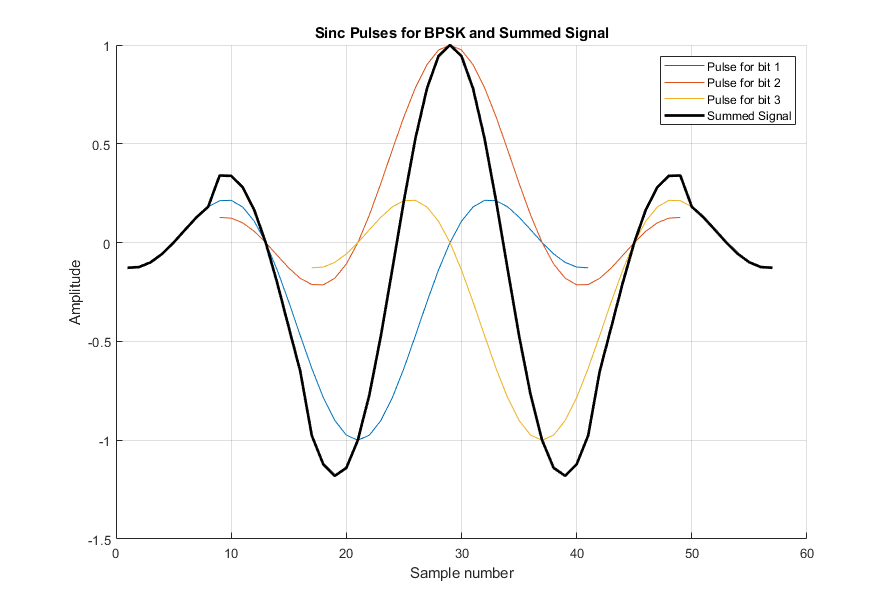
\includegraphics[width=\textwidth]{bpsk_signal_construction.png}
    \caption{Construction of the BPSK signal by summing sinc pulses for different bit combinations.}
\end{figure}


\subsection*{Receiver Scheme}

\subsubsection*{Matched Filter Design}
At the receiver, a matched filter is employed to maximize the signal-to-noise ratio (SNR) for the received signal. The concept of the matched filter arises from the need to optimize the correlation between the received signal and the filter's impulse response to maximize the output SNR. The impulse response \( h(t) \) of a matched filter is essentially the time-reversed and conjugated version of the signal's pulse shaping function \( s(t) \), which for BPSK is a sinc function. Thus, the matched filter impulse response is given by:
\[ h(t) = s^*(-T - t) \]
For a real-valued sinc pulse, conjugation does not change the function, and since the sinc function is symmetric, time-reversal is also redundant. Therefore, the matched filter impulse response in a BPSK system can be represented as:
\[ h_{\text{matched}}(n) = \text{sinc}\left(\frac{n}{T_s}\right) \]
where \( n \) is the discrete time index and \( T_s \) is the symbol period.

\subsubsection*{Signal Detection and Sampling}
To accurately decode the transmitted symbols, the matched filter output must be sampled at precise instants. The optimal sampling instants correspond to the peak response of the filter, which for a sinc pulse occurs at the center of the pulse. Given a symbol period of \( T_s \) and an oversampling factor \( n_{\text{shift}} \), the sampling instants are:
\[ n_{\text{sample}} = (i - 1) \cdot n_{\text{shift}} + \frac{n_{\text{shift}}}{2} \]
where \( i \) is the symbol index.

\subsubsection*{Bit Decision and Thresholding}
In BPSK, the received bit value is determined by the sign of the sampled matched filter output. For a positive sample, a bit value of 1 is assigned, while a negative sample indicates a bit value of 0. The decision rule can be expressed as:
\[ b_{\text{decoded}}[i] = 
\begin{cases}
1 & \text{if } y(n_{\text{sample}}) > 0, \\
0 & \text{otherwise},
\end{cases}
\]
where \( y(n_{\text{sample}}) \) is the matched filter output at the sampling instant. In the presence of noise, the sampled values may shift, necessitating an adjustment in the detection threshold. A zero threshold is assumed in the absence of explicit threshold setting in the code.

\subsubsection*{Convolution and Matched Filtering}
The process of matched filtering can be understood as the convolution of the received signal \( x(t) \) with the matched filter impulse response \( h(t) \):
\[ y(t) = x(t) * h(t) \]
The convolution operation in discrete-time for a signal \( x[n] \) and filter \( h[n] \) is defined as:
\[ y[n] = \sum_{k=-\infty}^{\infty} x[k] \cdot h[n - k] \]
This operation correlates the received signal with the time-reversed template of the transmitted pulse, thereby maximizing the SNR at the sampling instants.

\subsubsection*{Demodulation and BER Calculation}
The demodulation process involves filtering the received signal with the matched filter and sampling at the correct instants to determine the transmitted bit values. The function \texttt{decode\_bpsk\_signal} implements this process, filtering the received BPSK signal and sampling it to reconstruct the bit sequence. The bit error rate (BER) is evaluated by comparing the decoded bits to the original transmitted bits, quantifying the performance of the communication system.


\section*{Results}

\subsection*{Transmitted BPSK Signal}
The transmitted BPSK signal in the time domain is illustrated in Figure \ref{fig:bpsk_time}. The plot shows the binary data represented as BPSK values, where binary '0' is mapped to -1 and binary '1' is mapped to +1, demonstrating the phase shifts that encode the binary information.

\begin{figure}[h!]
    \centering
    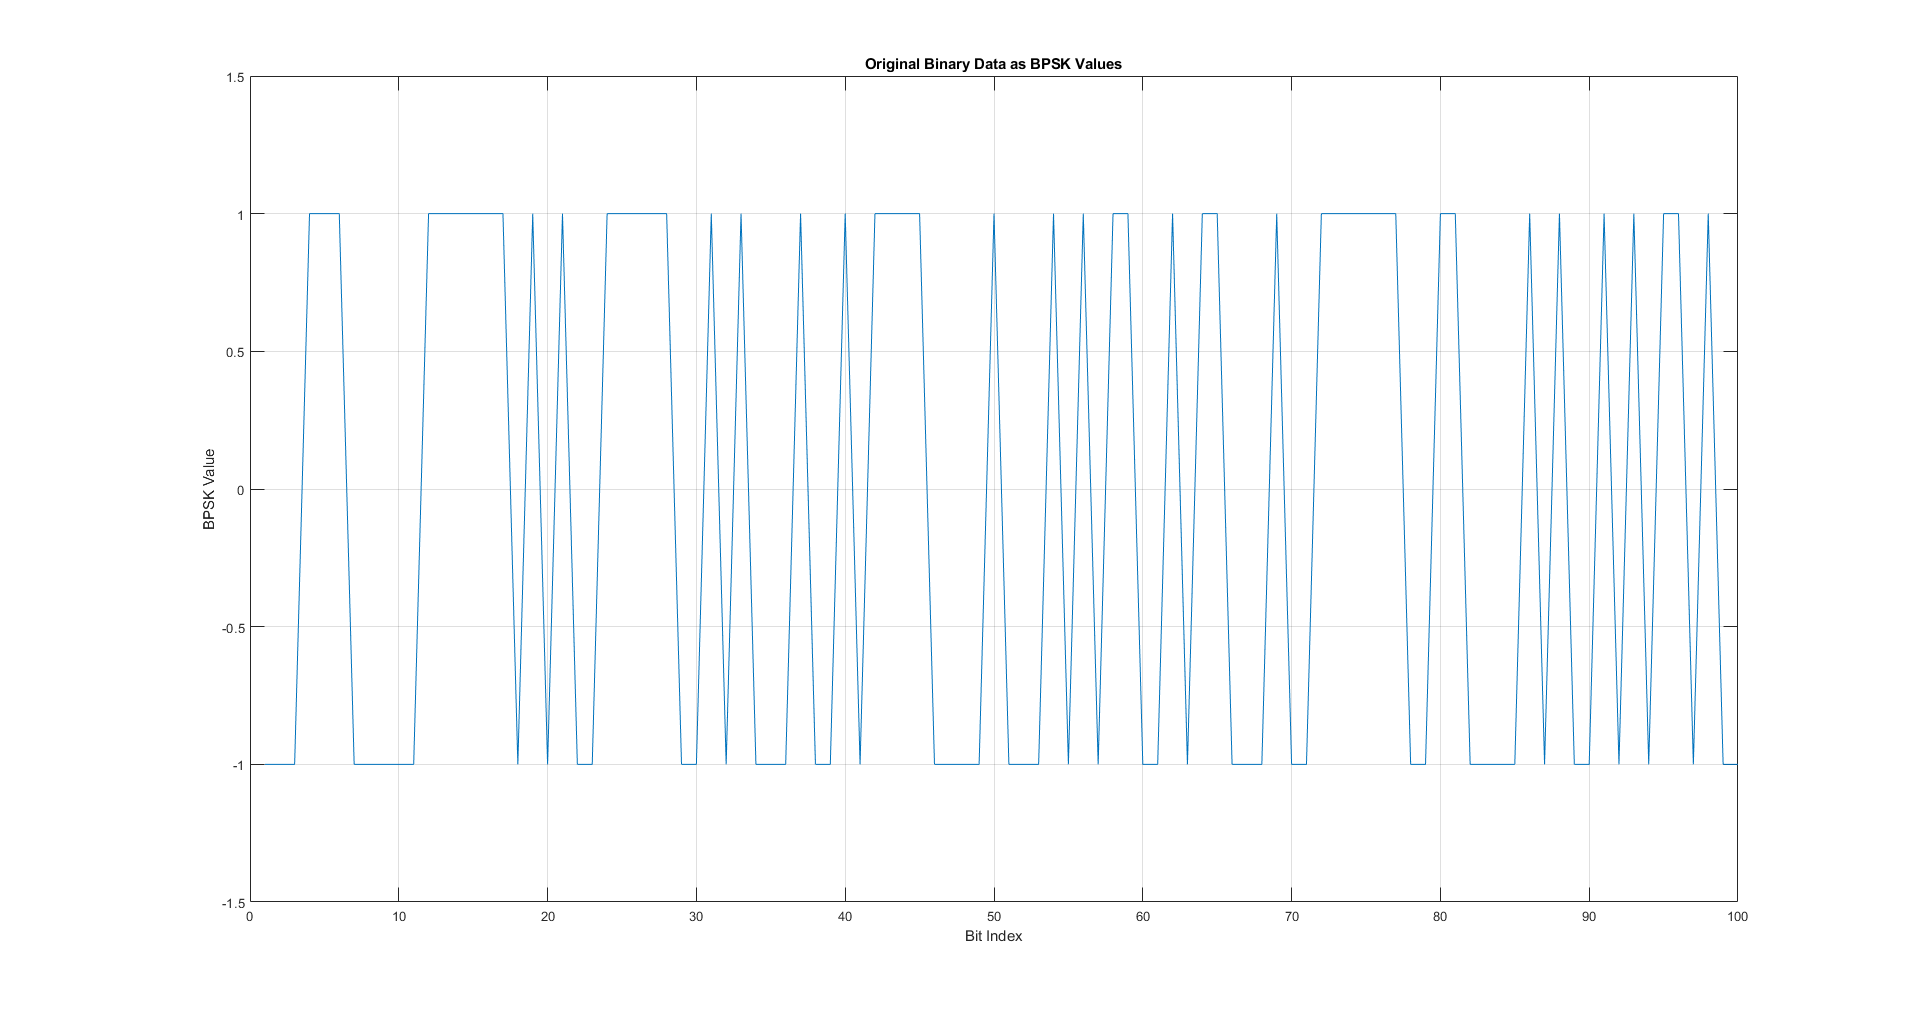
\includegraphics[width=\textwidth]{Binary_BPSK_Values.png}
    \caption{Original binary data represented as BPSK values in the time domain.}
    \label{fig:bpsk_time}
\end{figure}

\subsection*{Power Spectral Density of Transmitted Signal}
Figure \ref{fig:bpsk_psd} shows the Power Spectral Density (PSD) of the transmitted BPSK signal. The 3dB bandwidth is found to be approximately 200kHz, which is consistent across multiple runs of the simulation.

\begin{figure}[h!]
    \centering
    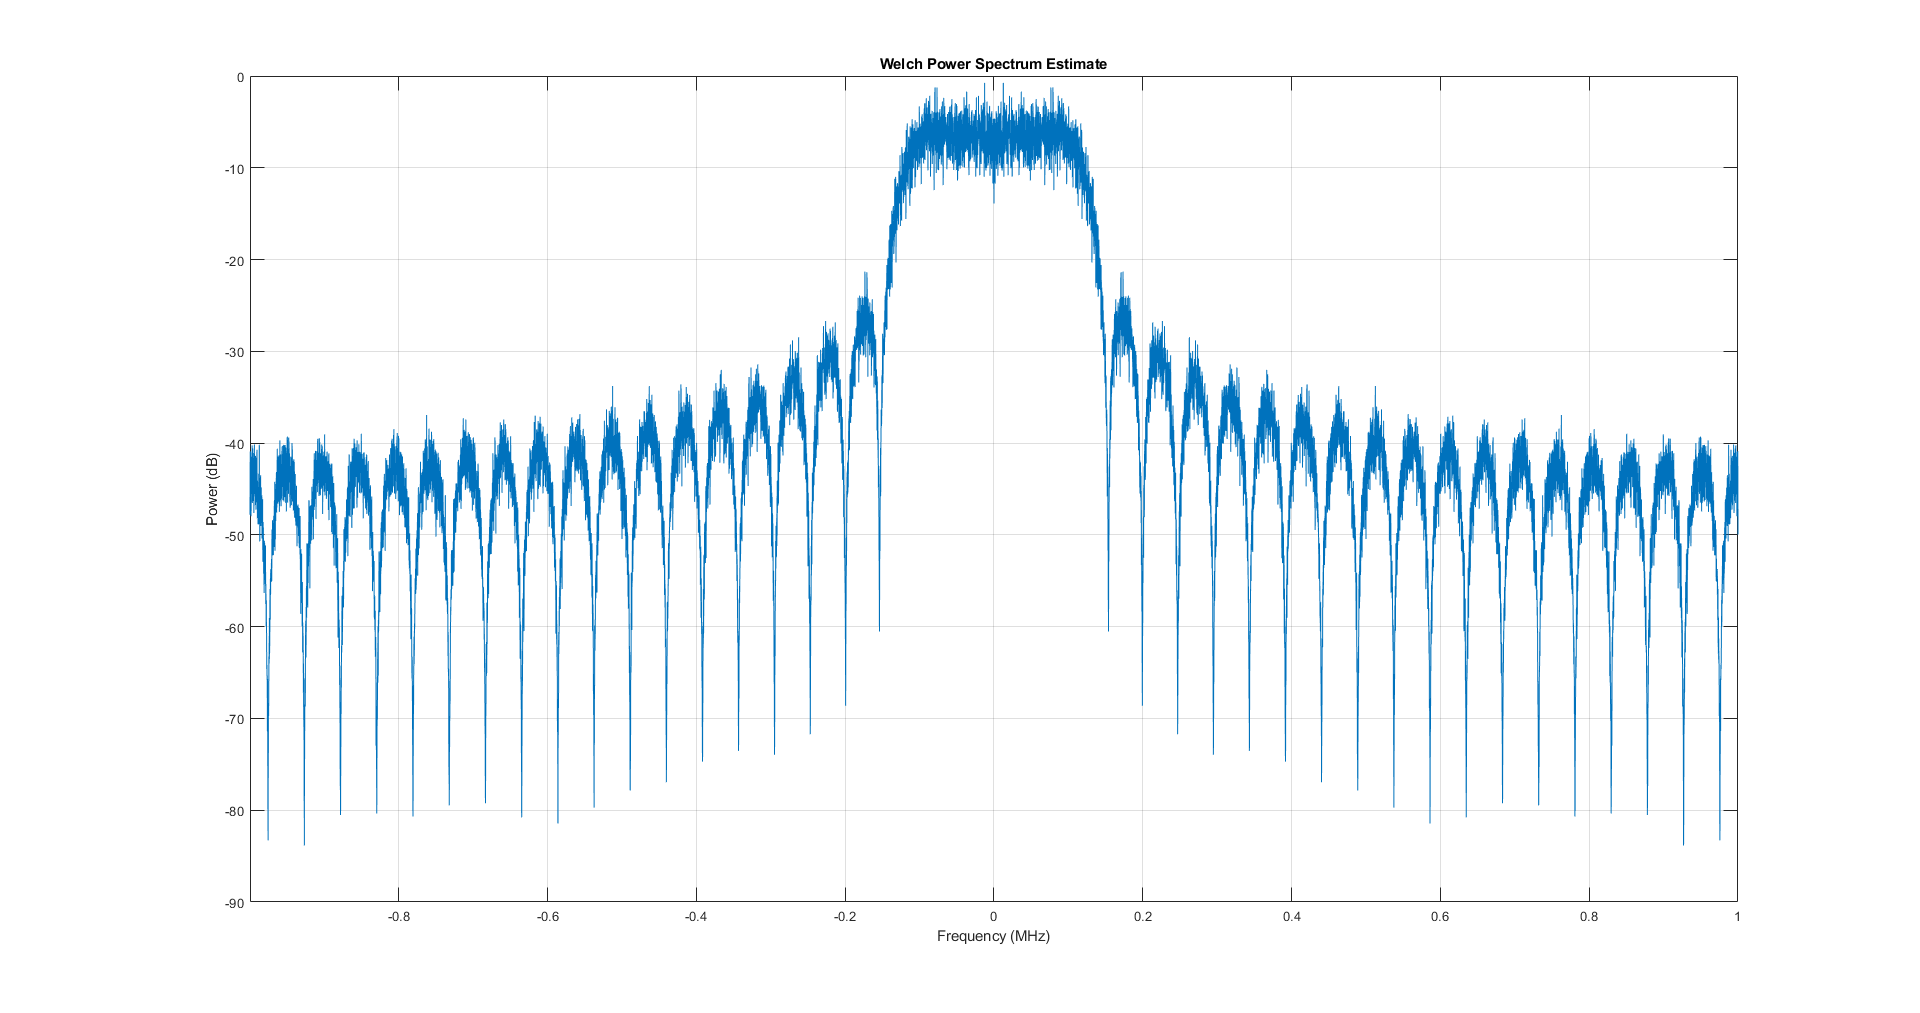
\includegraphics[width=\textwidth]{PSD_signal.png}
    \caption{Welch Power Spectrum Estimate of the transmitted BPSK signal.}
    \label{fig:bpsk_psd}
\end{figure}

The non-rectangular shape of the PSD is due to the practical implementation of the sinc pulse shaping, which in real systems cannot be infinitely long, leading to a "sinc squared" shape in the frequency domain.

\subsection*{Received and Processed Signals}
The summed BPSK signal before transmission is shown in Figure \ref{fig:summed_bpsk}, which demonstrates the superposition of individual sinc pulses that construct the entire signal.
\newline \newline
Figure \ref{fig:bpsk_noise} shows the received BPSK signal with added noise, illustrating the effect of the channel noise on the signal.

\begin{figure}[h!]
    \centering
    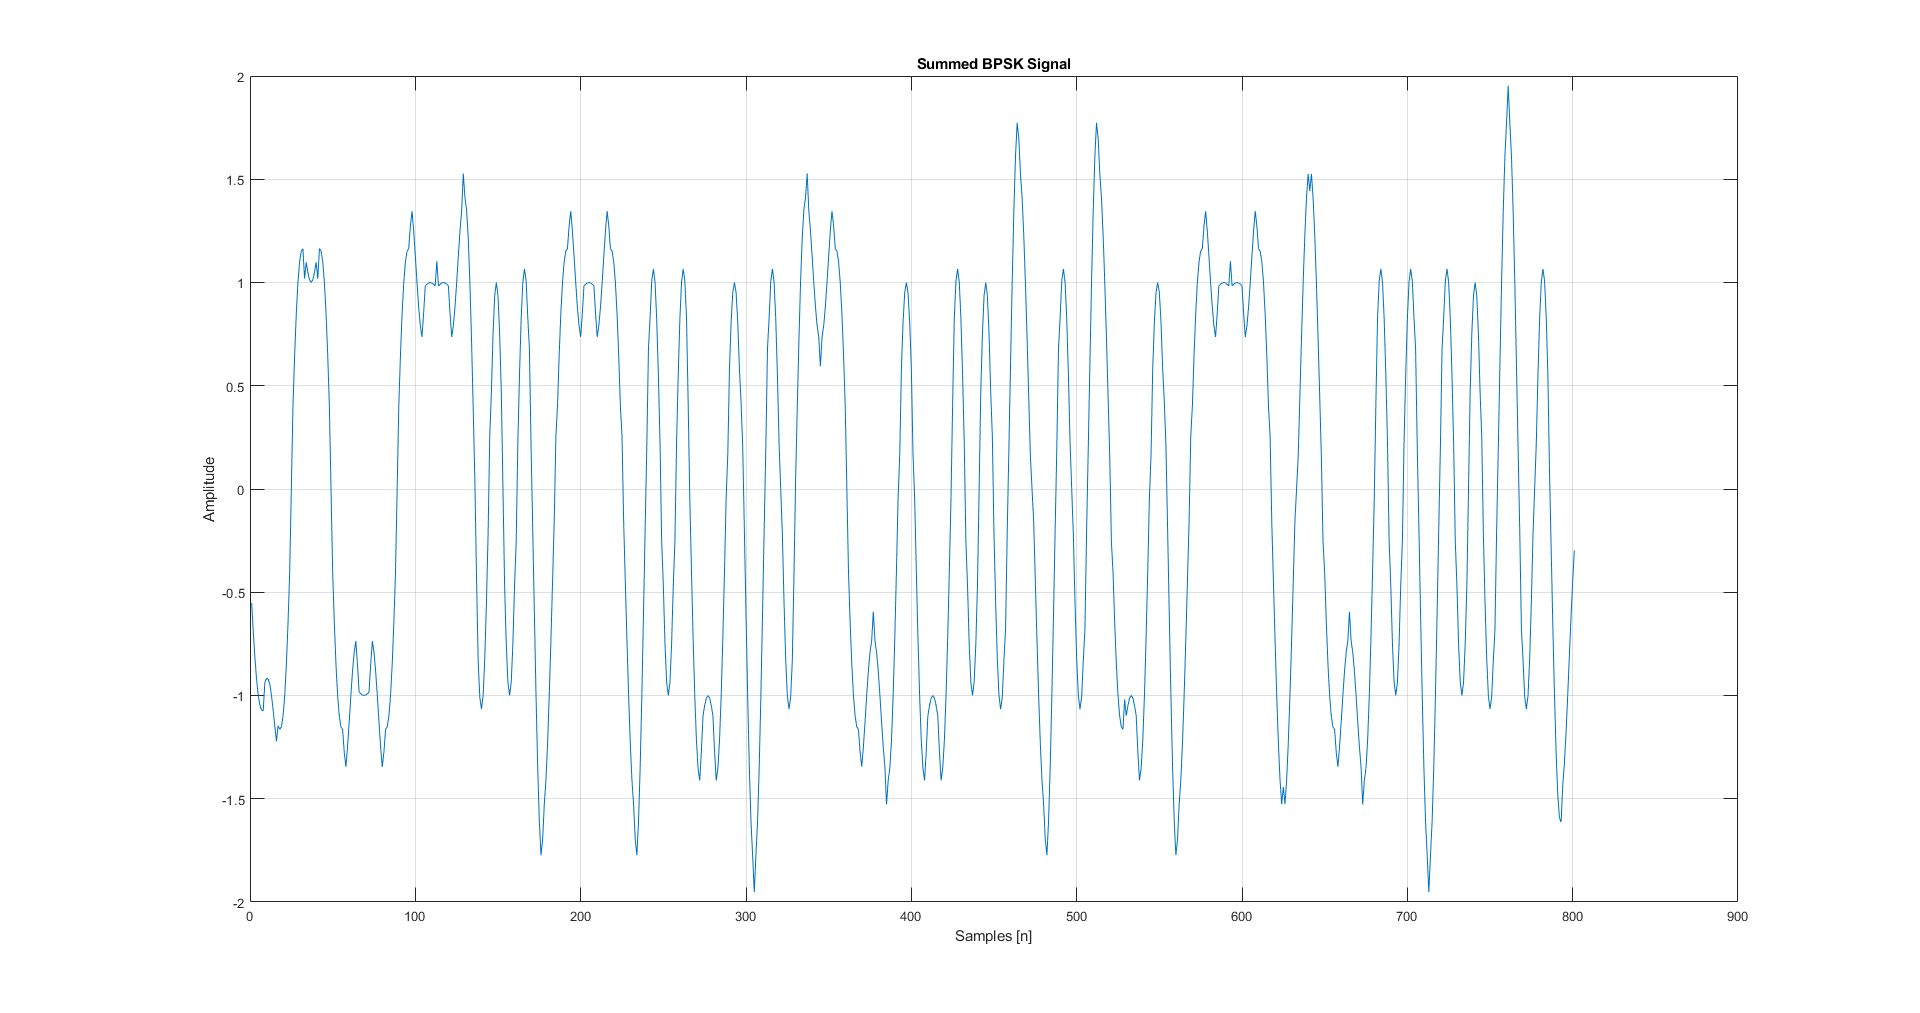
\includegraphics[width=\textwidth]{Summed_BPSK_Signal.png}
    \caption{Summed BPSK signal in the time domain before transmission.}
    \label{fig:summed_bpsk}
\end{figure}

\begin{figure}[h!]
    \centering
    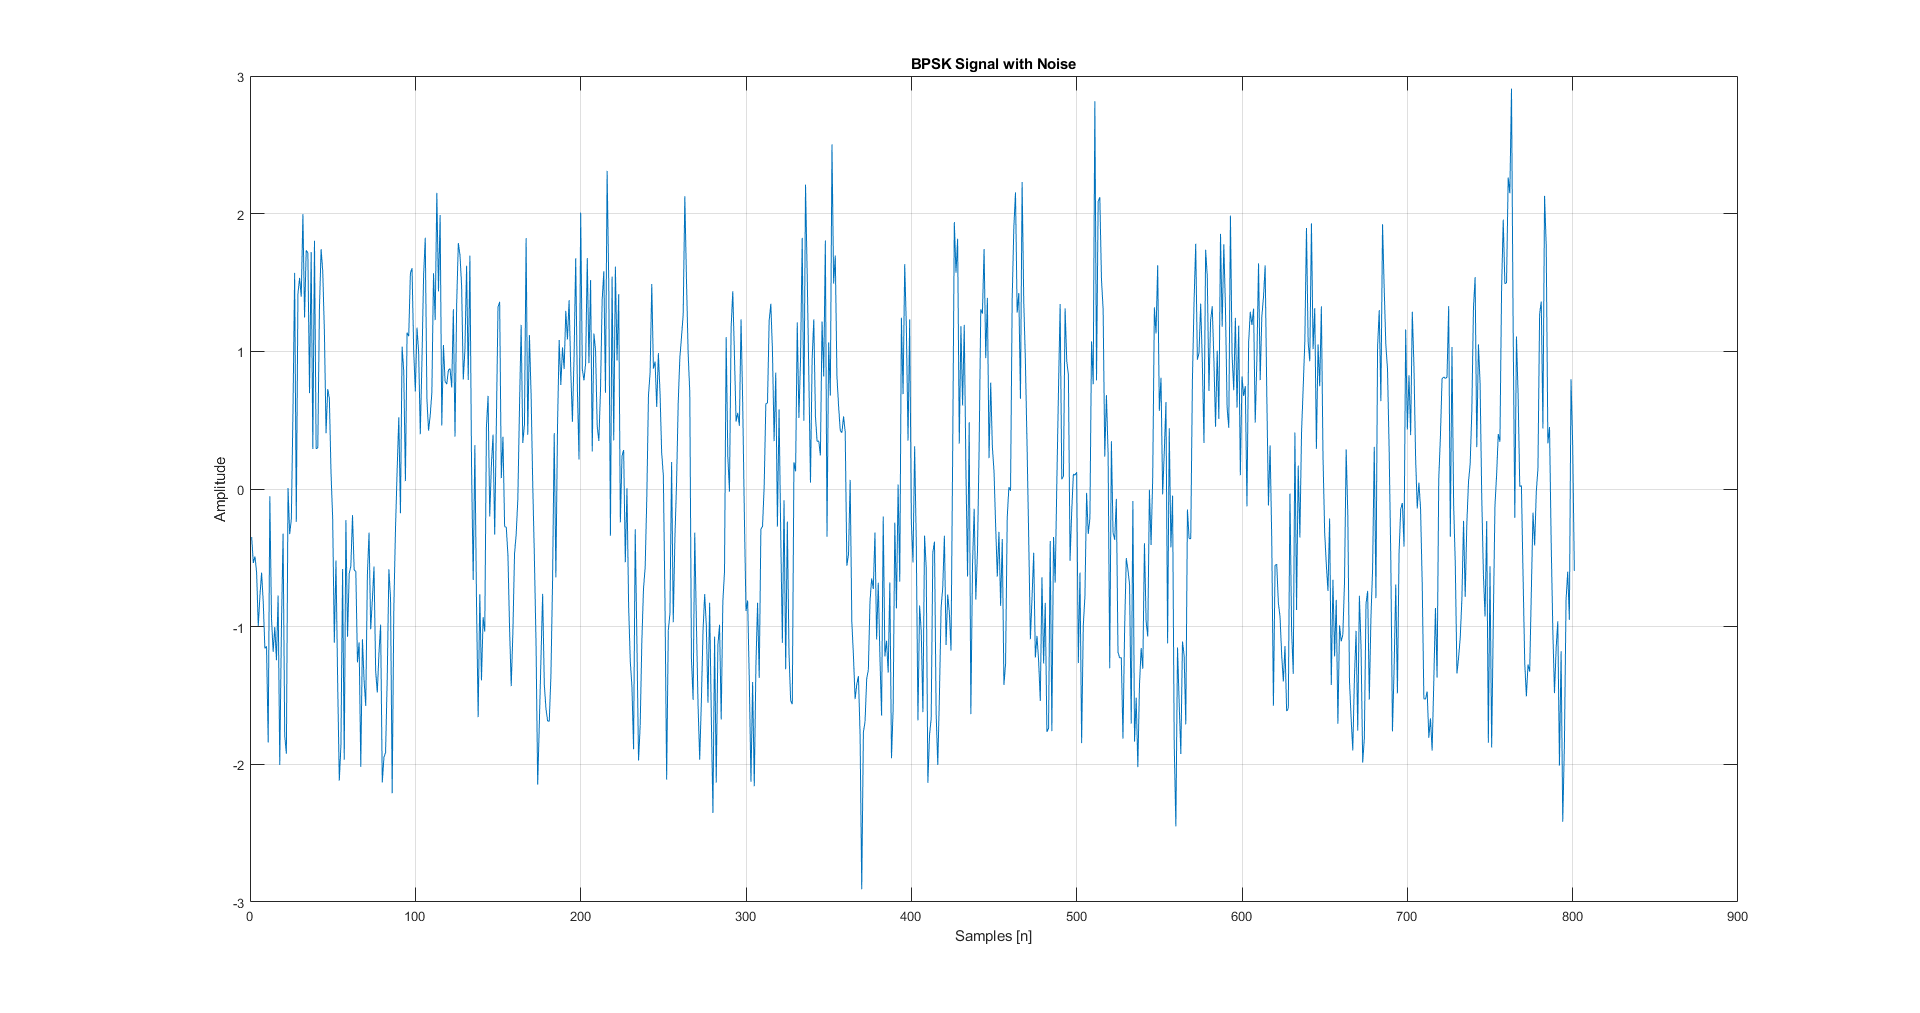
\includegraphics[width=\textwidth]{BPSK_Signal_with_Noise.png}
    \caption{BPSK signal with added noise in the time domain.}
    \label{fig:bpsk_noise}
\end{figure}

The filtered received signal, which is the output after the matched filter, with and without noise, is displayed in Figure \ref{fig:filtered_signal} and Figure \ref{fig:filtered_noise_signal}, respectively.

\begin{figure}[h!]
    \centering
    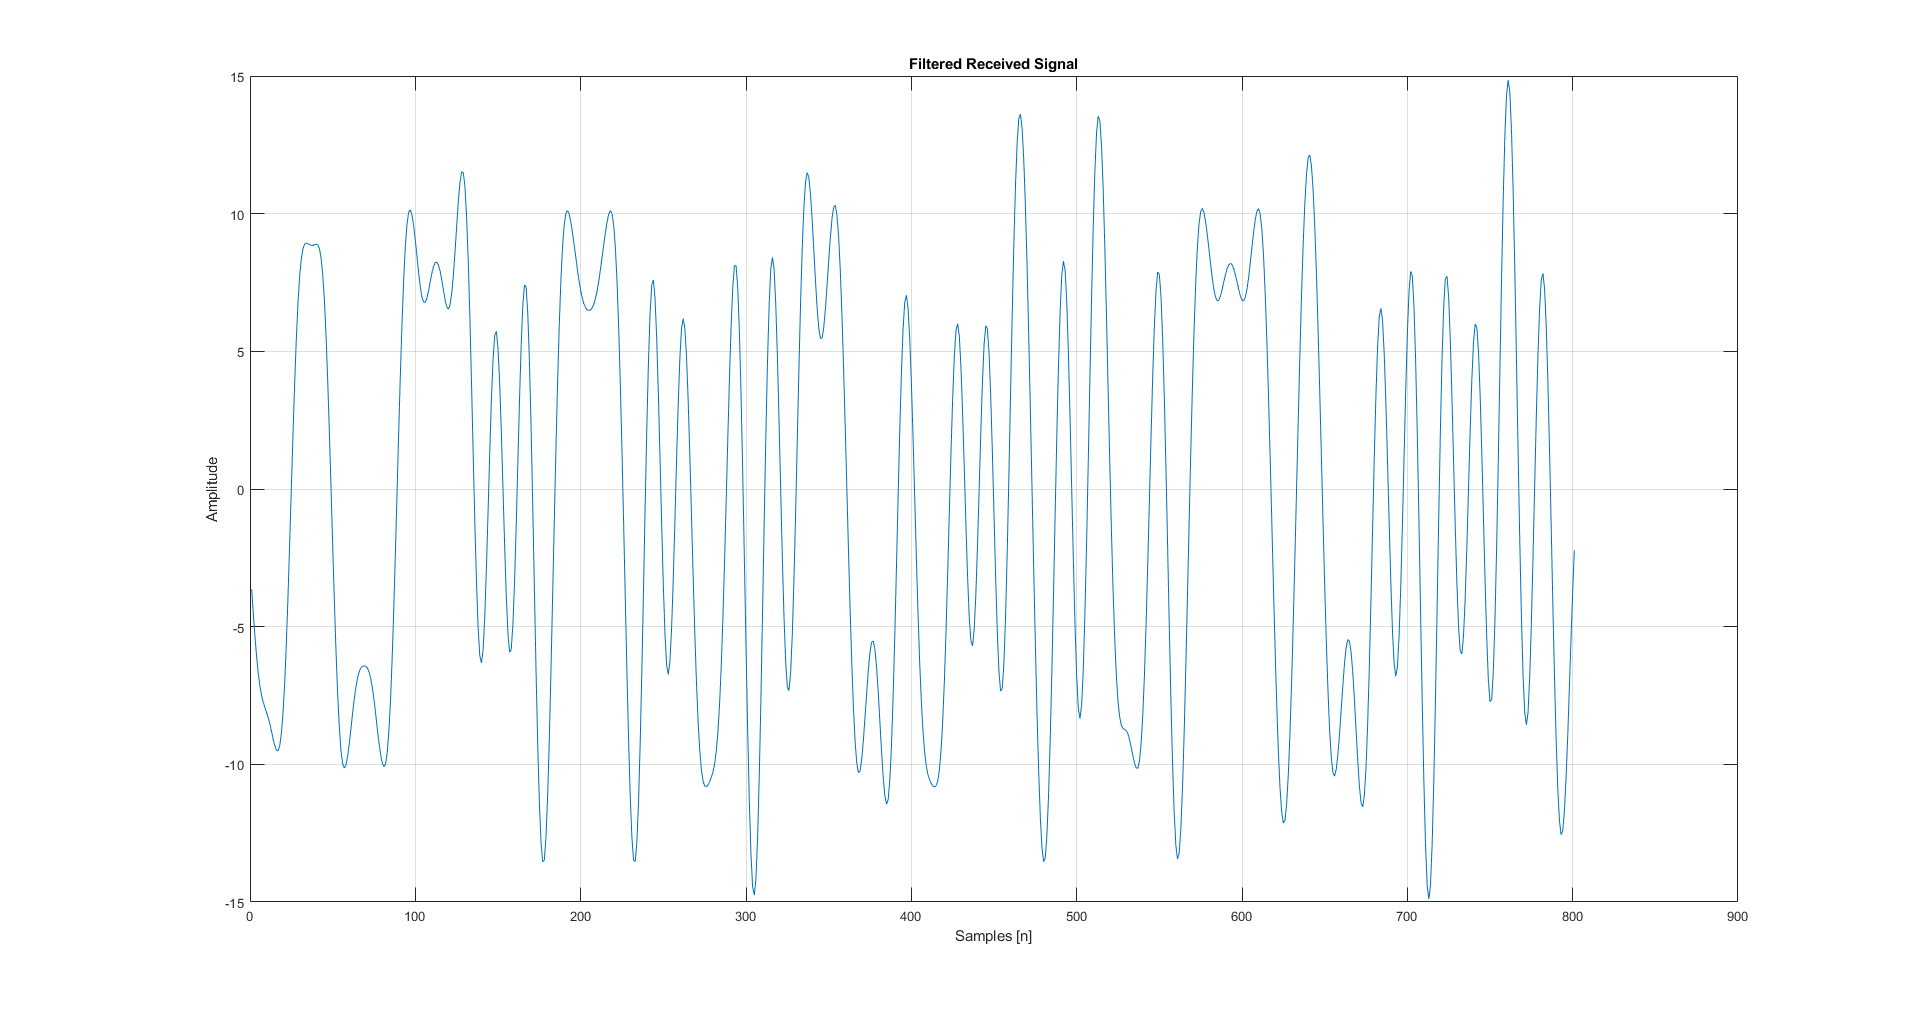
\includegraphics[width=\textwidth]{Filtered_Received_Signal.png}
    \caption{Filtered received BPSK signal without noise.}
    \label{fig:filtered_signal}
\end{figure}

\begin{figure}[h!]
    \centering
    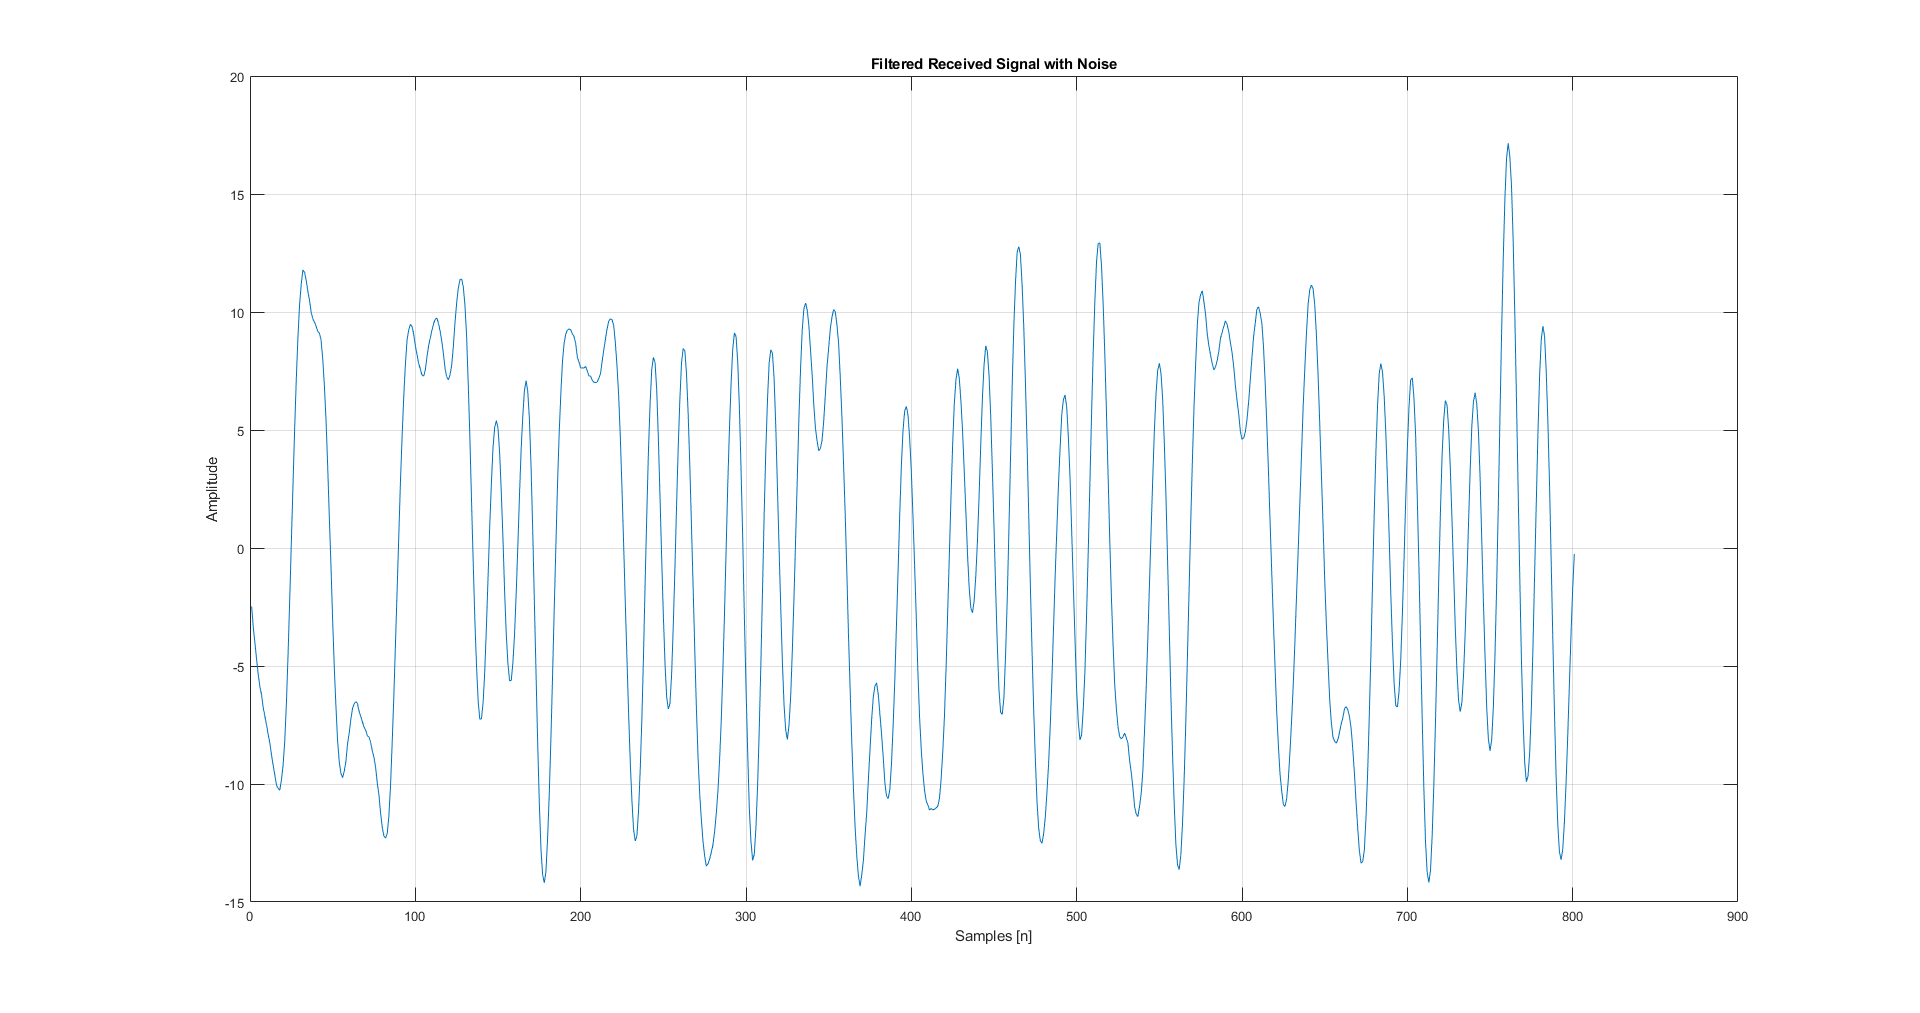
\includegraphics[width=\textwidth]{Filtered_Received_Signal_with_Noise.png}
    \caption{Filtered received BPSK signal with noise.}
    \label{fig:filtered_noise_signal}
\end{figure}

\subsection*{BER Performance}
Figure \ref{fig:ber_curve} presents the Bit Error Rate (BER) performance curve, comparing the simulation results with theoretical predictions. The graph indicates how the BER decreases with increasing Eb/N0, demonstrating the effectiveness of the BPSK modulation and demodulation process under varying noise conditions.

\begin{figure}[h!]
    \centering
    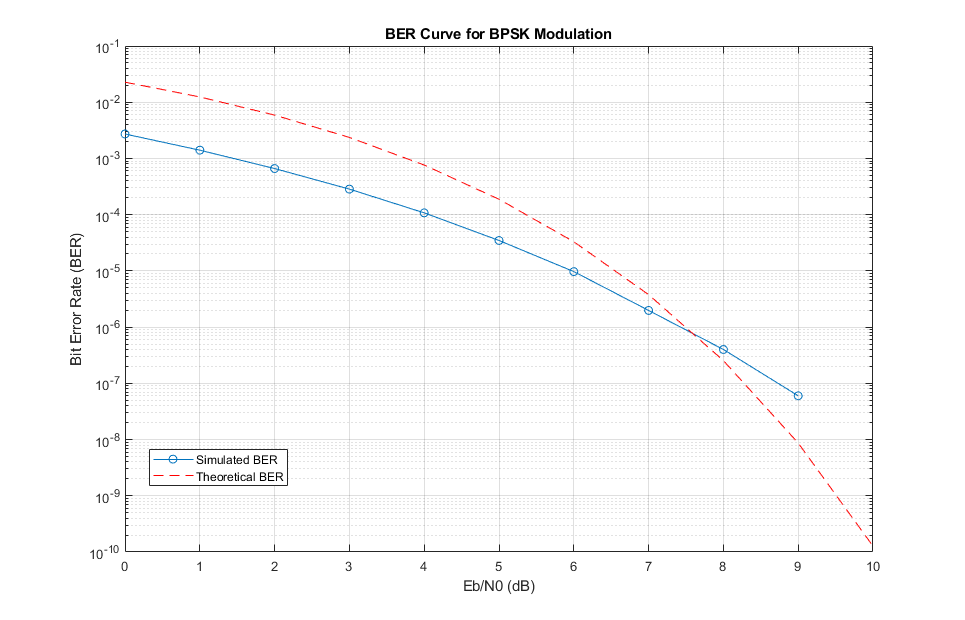
\includegraphics[width=0.8\textwidth]{BER_vs_SNR.png}
    \caption{BER Curve for BPSK Modulation comparing simulated and theoretical BER.}
    \label{fig:ber_curve}
\end{figure}

The analysis of the BER curve reveals that the simulated BER closely follows the theoretical predictions, indicating a well-modeled system that accounts for the noise effects accurately.

\subsection*{BER Results for Different \( E_b/N_0 \) Values}
The system's performance was evaluated for two different \( E_b/N_0 \) values, one on a linear scale and one in decibels (dB). 100 tests were run for each EBN0 value, each with 1e6 samples. The results are as follows:

\subsubsection*{\( E_b/N_0 \) = 2 (Linear Scale)}
For an \( E_b/N_0 \) value of 2 on a linear scale, the BER performance varied across different runs, with the best observed BER being 0.0002, the worst BER being 0.000278, and the average BER calculated to be 0.00024359. These results indicate a highly reliable system performance at this \( E_b/N_0 \) value.

\subsubsection*{\( E_b/N_0 \) = 2 dB}
When \( E_b/N_0 \) was set to 2 dB, the system showed a slightly higher BER compared to the linear scale. The best BER recorded was 0.000508, the worst BER was 0.000632, and the average BER was found to be 0.00058035. Although the BER is higher at this \( E_b/N_0 \) value, it still represents a reasonably low error rate, showcasing the robustness of the BPSK modulation scheme under this noise level.

\subsection*{Discussion on BER Results}
The observed variations in BER at different \( E_b/N_0 \) values are indicative of the system's sensitivity to the signal-to-noise ratio. As expected, an increase in \( E_b/N_0 \) improves the BER. The results demonstrate the trade-off between signal power and noise level, further emphasizing the importance of choosing an appropriate \( E_b/N_0 \) for reliable communication. The consistency between the best, worst, and average BER values suggests a stable system performance with little deviation between runs.



\section*{Additional Sections}
\subsection*{Combined Plots}
\subsubsection*{Comparison of Original, Filtered, and Noise-Affected BPSK Signals}
Figure \ref{fig:original_filtered_noise_signals} provides a comparative analysis of the original binary data represented in BPSK format, the filtered received signal, and the filtered received signal with noise. The original BPSK signal is shown to maintain distinct levels corresponding to the binary '0' and '1' values. After passing through the matched filter, the received signal retains its integrity with slight smoothing of the transitions between bit intervals. However, once noise is introduced, the signal's amplitude and phase are perturbed, which could potentially lead to bit errors if not properly mitigated by the receiver processing algorithms.

\begin{figure}[h!]
    \centering
    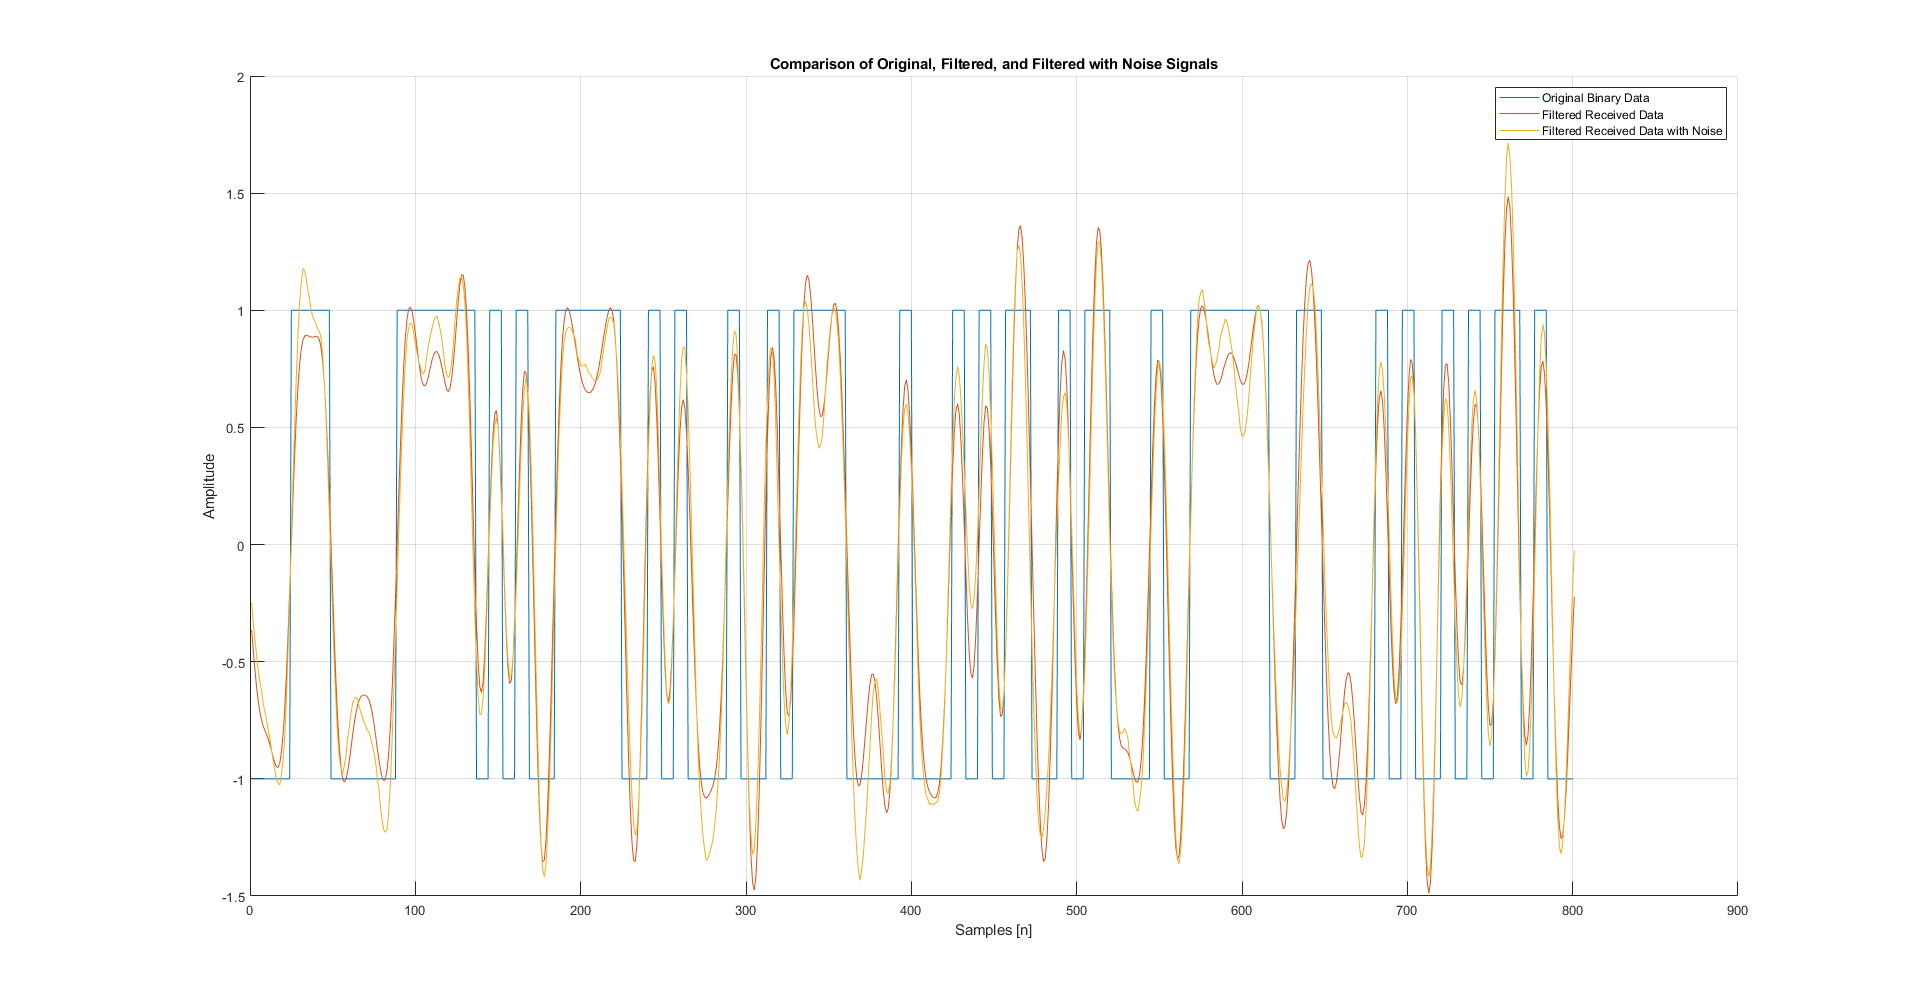
\includegraphics[width=\textwidth]{Combined_Original_Filtered.png}
    \caption{Comparison of the original BPSK signal, filtered received data, and filtered received data with noise.}
    \label{fig:original_filtered_noise_signals}
\end{figure}

\subsubsection*{Effect of Noise on BPSK Signal}
In Figure \ref{fig:bpsk_noise_effect}, the impact of noise on the BPSK signal is further examined. The overlay of the noise-free BPSK signal, the noise signal, and the composite signal demonstrates the nature of the noise interference. It is apparent from the plot that the noise induces significant fluctuations in the signal amplitude, which underscores the importance of a robust demodulation process to accurately recover the transmitted information.

\begin{figure}[h!]
    \centering
    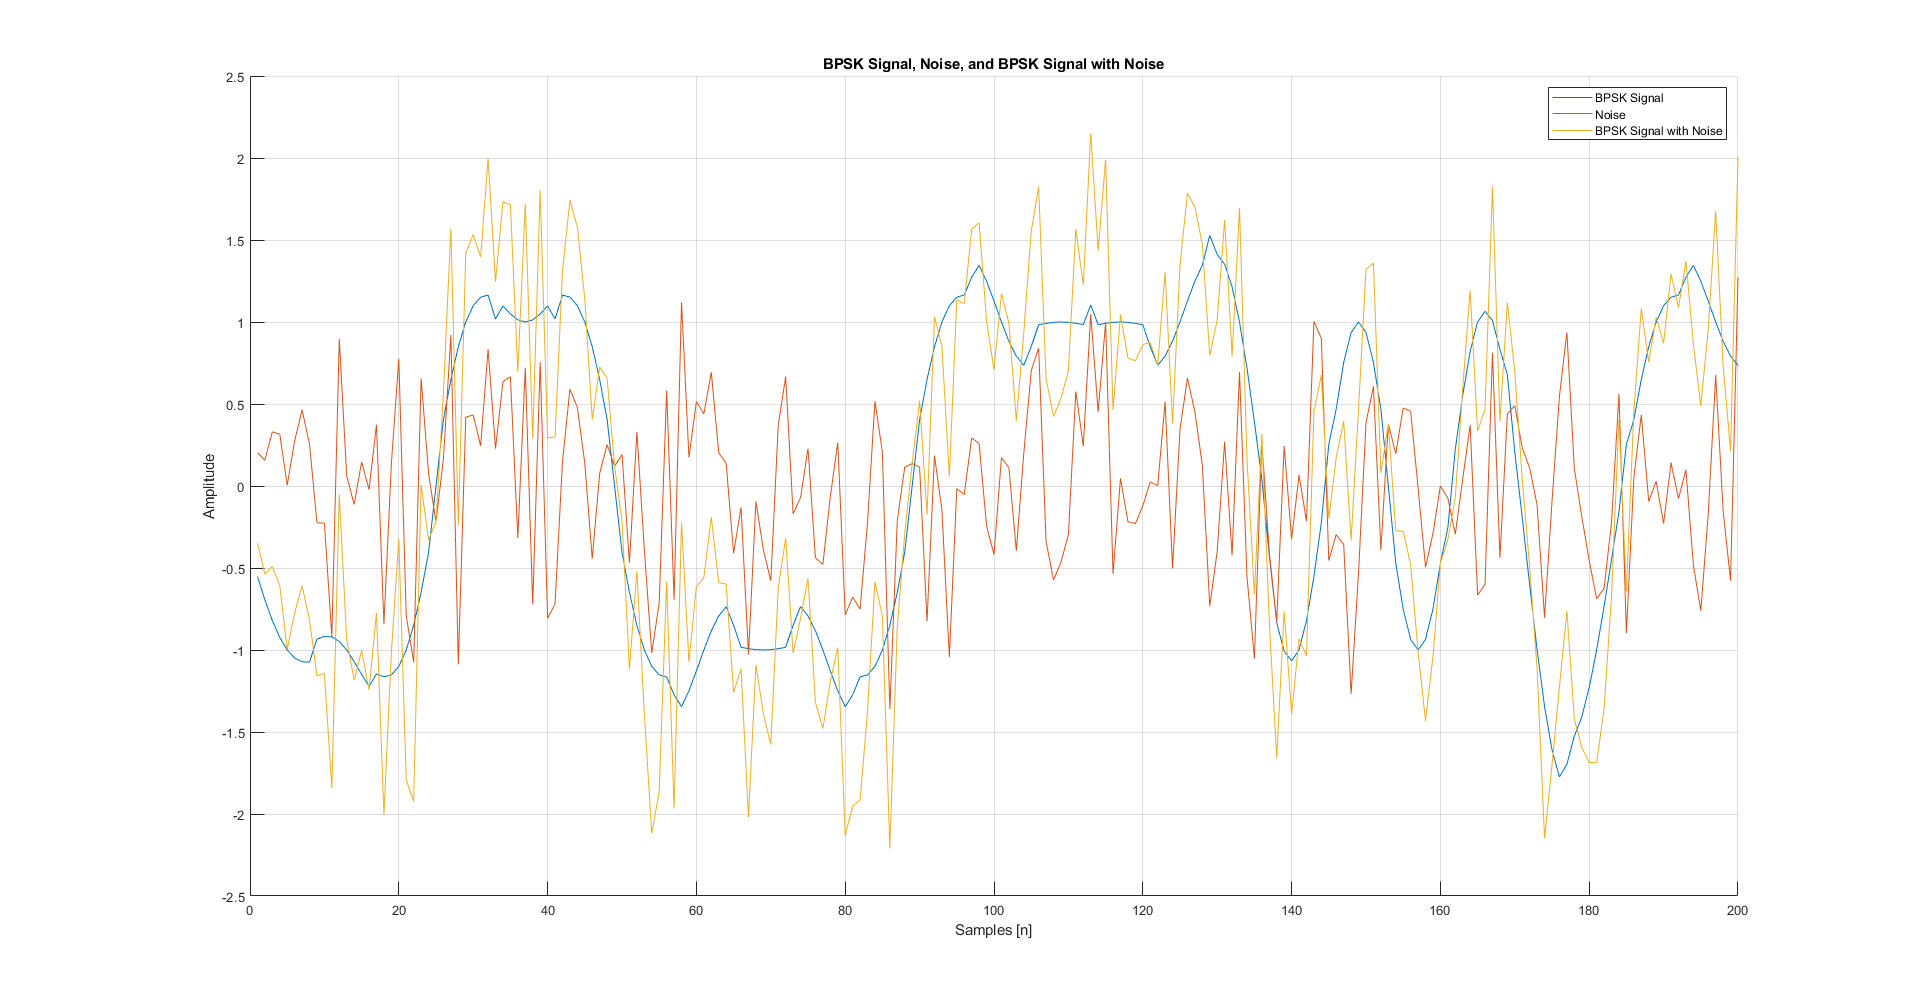
\includegraphics[width=\textwidth]{Combined_BPSK_Noise.png}
    \caption{BPSK signal, noise signal, and BPSK signal with superimposed noise in the time domain.}
    \label{fig:bpsk_noise_effect}
\end{figure}

These detailed analyses underscore the challenges posed by noise in communication systems and the necessity for effective filtering and demodulation techniques to ensure signal integrity and reliability.


\section*{Code Optimization Process}
The generation of a BPSK signal from a binary array was optimized over three versions of a MATLAB function, with each subsequent version significantly reducing the computation time. The final version was ten times faster than the original and three times faster than its predecessor.

\subsection*{Version 1 to Version 2}
The first optimization from Code v1 to Code v2 involved the precomputation of the sinc pulse. In Code v1, the sinc function was defined as a lambda function and recalculated for every bit in the binary array, whereas in Code v2, the sinc pulse was computed once before the loop. This change eliminated redundant calculations and reduced the number of function calls, leading to a tenfold increase in speed.

\subsection*{Version 2 to Version 3}
The second optimization from Code v2 to Code v3 capitalized on the convolution properties of signals. Instead of manually shifting and adding sinc pulses for each bit, Code v3 created an upsampled BPSK values array with zeros in between to match the sinc pulse rate. The convolution of the entire upsampled array with the sinc pulse was then performed in a single step using MATLAB's built-in \texttt{conv} function. By leveraging the efficiency of MATLAB's optimized convolution operation, the code was made three times faster than Code v2.

\subsection*{Discussion}
The original code performed individual calculations for each bit, resulting in inefficient use of both time and computational resources. By precomputing common values and utilizing array operations, the optimized versions reduced the computational load. The final version, Code v3, improved performance by exploiting the fact that convolution is a more computationally efficient operation when dealing with signal processing in MATLAB, especially when the signals are represented in arrays. This optimization process not only sped up the computation but also made the code more readable and concise.


\section*{Visualization of Sinc Pulses in BPSK Signal Generation}

\subsection*{Functionality of plot\_sinc\_pulses}
The function \texttt{plot\_sinc\_pulses} provides a visual representation of how individual sinc pulses, corresponding to each bit in a binary array, contribute to the overall BPSK signal. The function initializes an array to hold the sum of all sinc pulses, and then iteratively generates and plots each sinc pulse based on the binary data. Pulses corresponding to a binary '1' are plotted with an amplitude of 1, while those corresponding to a binary '0' are inverted, with an amplitude of -1. The function also plots the aggregate of all pulses to illustrate the final BPSK signal waveform.

\subsection*{Importance of Visualization}
Visualizing the sinc pulses is critical for several reasons:

\begin{itemize}
    \item \textbf{Understanding Signal Construction:} It helps in understanding how a BPSK signal is constructed from individual pulses, showing the role of each bit in shaping the signal.
    \item \textbf{Time-domain Insights:} Observing the signal in the time domain provides insights into the modulation process, particularly how the phase of the carrier wave is modulated by the binary data.
    \item \textbf{Debugging and Verification:} For educational purposes or in the process of designing a modulation scheme, being able to visually inspect the intermediate steps of signal generation is invaluable for debugging and verification.
    \item \textbf{Impact of Signal Parameters:} The effect of parameters such as sample number and shift between pulses can be clearly seen, allowing for a deeper understanding of how these parameters affect the bandwidth and shape of the BPSK signal.
\end{itemize}

\subsection*{Graphical Output}
The function generates a plot that includes each sinc pulse and the summed signal. The individual pulses are labeled for clarity, and the summed signal is emphasized with a thicker line. The use of legend and grid enhances the readability of the plot, making it an effective tool for both teaching and analysis.

This visual aid is not only an educational resource but also a practical tool for signal processing engineers to verify the integrity of the BPSK signal generation process.


\section*{Eb/N0 Simulation Code Explanation}

The \texttt{EB\_N0\_Simulation} function in MATLAB is designed to simulate the Bit Error Rate (BER) for a Binary Phase Shift Keying (BPSK) modulation scheme over a range of energy per bit to noise power spectral density ratio (Eb/N0) values.

\subsection*{Function Definition}
\begin{verbatim}
function EB_N0_Simulation(step_size, num_bits)
\end{verbatim}
This function takes two parameters: \texttt{step\_size}, which determines the increment in the Eb/N0 value for each simulation step, and \texttt{num\_bits}, the total number of bits to be simulated.

\subsection*{Simulation Process}
\begin{itemize}
    \item The Eb/N0 range is defined from 0 dB to 10 dB.
    \item Arrays to store the simulated and theoretical BER are initialized.
    \item Random binary data of length \texttt{num\_bits} is generated.
    \item The binary data is modulated using an optimized BPSK signal generation function.
    \item Noise variance for each Eb/N0 value is pre-calculated.
    \item The theoretical BER is computed using the complementary error function (\texttt{erfc}) over the square root of twice the signal-to-noise ratio (SNR).
    \item A loop (or parallel loop with \texttt{parfor} for large simulations) iterates over each Eb/N0 value, adding corresponding Gaussian noise to the modulated signal, demodulating it, and computing the simulated BER.
\end{itemize}

\subsection*{Performance Bottleneck}
The simulation can become computationally intensive with a large number of bits due to the following factors:
\begin{itemize}
    \item Generation of Gaussian noise for each bit at each Eb/N0 value.
    \item The demodulation process, which involves comparison for each bit to determine errors.
\end{itemize}
For simulations with a high bit count (e.g., over $10^6$ bits), it is recommended to use MATLAB's parallel processing capabilities with \texttt{parfor} to enhance computation speed.

\subsection*{Output}
The function plots the simulated BER against the theoretical BER on a semi-logarithmic scale, providing a visual comparison of the system's performance under different noise levels.

\subsection*{Conclusion}
\begin{verbatim}
semilogy(EbN0_dB, BER_simulated, 'o-', 'DisplayName', 'Simulated BER');
semilogy(EbN0_dB, BER_theoretical, 'r--', 'DisplayName', 'Theoretical BER');
\end{verbatim}
The \texttt{EB\_N0\_Simulation} function concludes by plotting the BER performance, which is crucial for understanding the reliability of the BPSK modulation scheme in a noisy communication channel.


\section*{MATLAB Code Implementation}

The following sections contain the MATLAB code used in the simulation and analysis of the BPSK communication system.

\subsection*{generate\_bpsk\_signal\_optimized2.m}
\lstinputlisting[language=Matlab]{generate_bpsk_signal_optimized2.m}

\subsection*{decode\_bpsk\_signal.m}
\lstinputlisting[language=Matlab]{decode_bpsk_signal.m}

\subsection*{primary\_code\_CA8.m}
\lstinputlisting[language=Matlab]{primary_code_CA8.m}

\subsection*{EBN0\_2\_test.m}
\lstinputlisting[language=Matlab]{EBNO_2_test.m}

\subsection*{EB\_N0\_Simulation.m}
\lstinputlisting[language=Matlab]{EB_N0_Simulation.m}

\subsection*{plot\_sinc\_pulses.m}
\lstinputlisting[language=Matlab]{plot_sinc_pulses.m}

\subsection*{additional\_figures.m}
\lstinputlisting[language=Matlab]{additional_figures.m}

\end{document}




\end{document}
